%%%%%%%%%%%%%%%%%%%%%%%%%%%%%%%%%%%%%%%%%%%%%%%%%%%%%%%%%%%%%%%%%%%%%%%%%%%%%%%
%
% results
% Copyright (c) 2010 by tilo.mueller@rwth-aachen.de
% 
%%%%%%%%%%%%%%%%%%%%%%%%%%%%%%%%%%%%%%%%%%%%%%%%%%%%%%%%%%%%%%%%%%%%%%%%%%%%%%%

\chapter{Ergebnisse}

TODO: Roadmap (erst am Ende, "Kapitel 4 unterteilt sich in ... Unterkapitel und ...)

\section{Demographie}
\label{sec:demo}
Die Studiendurchführung ergab 1020 beantwortet Fragebögen. Nach Bereinigung der Daten sind hieraus 856 vollständig bewertbare Fragebögen hervorgekommen. Entfernt wurden hierbei Fragebögen die nicht vollständig ausgefüllt waren oder abgebrochen wurden.

Von den 856 Teilnehmern waren 204 (23,8\%) weiblich, 613 (71,6\%) männlich und 39 haben keine Angabe zu ihrem Geschlecht gemacht. Die hohe Anzahl an männlichen Teilnehmern liegt vermutlich daran, dass die Umfrage über den E-Mail Verteiler der Technischen Fakultät der Universität Erlangen-Nürnberg verteilt wurde, welche einen höheren Männer- als Frauenanteil hat.

Im Mittelwert waren die Teilnehmer 25,0 Jahre alt. Interessant ist, dass trotz des niedrigen Wertes und der geringen Standardabweichung dennoch 47 Teilnehmer im Altersbereich von 45 bis 77 liegen. Die prozentuale Anzahl reicht dennoch nicht, um genaue statistische Aussagen über diese Gruppe im einzelnen zu treffen, deswegen wird auf eine spezielle Auswertung verzichtet.

Beim Bildungsabschluss zeigt sich dass ein Großteil der Teilnehmer entweder gerade studiert oder bereits einen Abschluss im Studium erreicht hat. Teilnehmer die ein Abitur oder einen Abschluss als Bachelor/Master/Diplom haben berechnen sich auf über 90\% der Teilnehmer. Nur knapp über 5,7\% der Befragten hatten einen Haupt- oder Realschulabschluss.

Somit spiegelt die demographische Verteilung der Studienteilnehmer nicht die Gesamtzahl der Google-Nutzer in Deutschland wieder, da 2014 60,7\% der Deutschen mit Volks-/Hauptschulabschluss das Internet genutzt haben \cite{statistabildung}. In einer zukünftigen Arbeit zu diesem Thema sollten eventuell speziell die Gruppen \glqq Kein Abschluss\grqq\ , \glqq Hauptschulabschluss\grqq\ und \glqq Realschulabschluss\grqq\ betrachtet werden.

\begin{figure}[H]
\centering
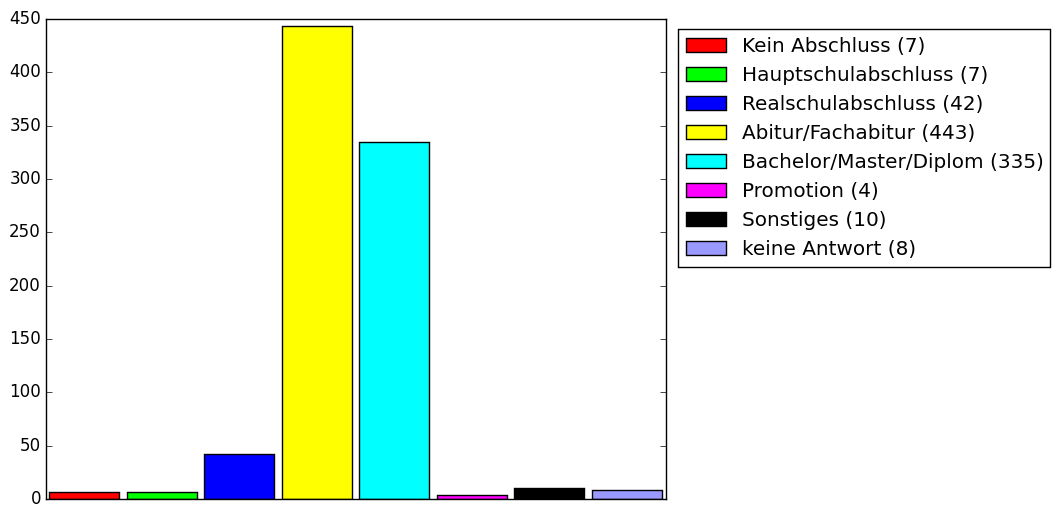
\includegraphics[scale=0.55]{images/schulabschluss}\\
\caption{Höchster Schulabschluss}\label{schulabschluss}
\end{figure}
Auch die Auswertungen zu der derzeitigen Arbeitsbeschäftigung zeigen ein ähnliches Bild - 77,0\% der Teilnehmer (659) waren zum Zeitpunkt der Studiendurchführung Studenten. Dahingegen sind nur 2,0\% in Ausbildung und 15,0\% berufstätig.

Das arithmetische Mittel der selbst eingeschätzten Informatikkenntnisse liegt auf einer Skala von 1 (keine) bis 5 (sehr hohe) bei 3,3. Hier wurde angenommen, dass im Durchschnitt ein Wert von 3,0 erreicht wird, da dies der Mittelwert der auszuwählenden Optionen war und man bei spezialisiertem Wissen von einer Normalverteilung, die ihr Maximum ungefähr in der Mitte hat, ausgehen kann. Dass dieser Wert sehr nah an dem von mir erwartetem Mittelwert von 3,0 liegt deutet darauf hin, dass die Umfrage trotz der geringen Anzahl an Realschülern und Hauptschülern dennoch Relevanz hat, wenn man weiterhin annimmt, dass der Wissenstand im Bereich Informatik hier der ausschlaggebende Faktor ist und nicht der Bildungsstand.

Diese Statistik verschiebt sich stark, wenn man die Frage nach den Kenntnissen in der IT-Sicherheit betrachtet. Hier liegt das arithmetische Mittel bei 2,6, was um 0,7 niedriger ist als das arithmetische Mittel der IT Kenntnisse.

In Tabelle \ref{4sitsecteach} lässt sich deutlich sehen, dass ein Bildungsabschluss in der Informatik sich auf die Kenntnisse im Bereich IT-Sicherheit auswirkt. Die prozentualen Angaben sind hier spaltenweise zu lesen - zum Beispiel schätzen 39,7\% derjenigen, die einen Abschluss im IT-Bereich haben ihre Kenntnisse im Bereich IT-Sicherheit auf eine 4 ein. Aus den prozentualen Angaben lässt sich schnell sehen, dass diejenigen, die keinen Abschluss im IT-Bereich haben sich zum Großteil auf der unteren Hälfte der IT-Sicherheit antragen, wohingegen es bei denjenigen mit Abschluss im Bereich 4 und 5 schon über 50\% der Teilnehmer eingetragen haben.
Die weiteren demographischen Ergebnisse sind der Übersichtlichkeit halber in Tabelle \ref{demoqna} zusammengefasst.\\
\begin{table}
	\begin{tabular}[]{ l c | c | c | c | c }
	& & \multicolumn{3}{c |}{Haben Sie einen Bildungsabschluss in der Informatik} &\\
	& & \multicolumn{3}{c |}{oder einem anderen IT-nahem Fachbereich?} &\\ \hline
	& & Ja & Nein & Gesamt\\ \hline
	Haben Sie Kenntnisse im Bereich& 1 & 3 (1,6\%) & 138 (20,9\%) & 141\\
	IT-Sicherheit?& 2 & 23 (12,5\%) & 238 (36,0\%) & 261\\
	(1: gar nicht, 5: sehr)& 3 & 59 (32,1\%) & 193 (29,2\%) & 252\\
	& 4 & 73 (39,7\%) & 78 (11,8\%) & 151\\
	& 5 & 26 (14,1\%) & 14 (2,1\%) & 40\\ \hline
	Gesamt & & 184 & 661 & 845\\ \hline
	\end{tabular}
	\caption{Haben Sie Kenntnisse im Bereich IT-Sicherheit? x Haben Sie einen Bildungsabschluss in der Informatik oder einem anderen IT-nahem Fachbereich?}\label{4sitsecteach}
\end{table}

\begin{table}
	\begin{tabular}[]{ l | l | c | c }
	\hline
	Frage & Antwort & Anzahl (absolut) & Anzahl (relativ) \\
	\hline
	& weiblich &  204 & 23,8\% \\
	Sind Sie:& männlich & 613 & 71,6\% \\
	& keine Antwort & 39 & 4,6\% \\
	\hline \hline
	& Kein Abschluss & 7 & 0,8\% \\
	& Hauptschulabschluss & 7 & 0,8\% \\
	& Realschulabschluss & 42 & 4,9\% \\
	Welchen höchsten Schulabschluss& Abitur/Fachabitur & 443 & 51,75\% \\
	haben Sie? & Bachelor/Master/Diplom & 335 & 39,1\% \\
	& Promotion & 4 & 0,5\% \\
	& Sonstiges & 10 & 1,2\% \\
	& keine Antwort & 8 & 1,0\% \\
	\hline \hline
	& In Ausbildung & 17 & 2,0\% \\
	& Student/-in & 659 & 77,0\% \\
	& Berufstätig & 127 & 15,0\%\\
	Sie sind derzeit: & In Rente & 4 & 0,5\% \\
	& Nicht Berufstätig & 19 & 2,2\% \\
	& Sonstiges & 23 & 2,7\% \\
	& keine Antwort & 7 & 0,8\% \\
	\hline \hline
	& 1 & 23 & 2,7\%\\
	& 2 & 205 & 24,2\% \\
	Wie hoch schätzen Sie ihre & 3 & 266 & 31,4\% \\
	Informatik Kenntnisse ein? & 4 & 239 & 28,2\% \\
	(1 = niedrig, 5 = sehr hoch)& 5 & 114 & 13,5\% \\
	& keine Antwort & 9 & 1,0\% \\
	\hline \hline
	& 1 & 143 & 16,8\% \\
	& 2 & 262 & 31,0\% \\
	Haben Sie Kenntnisse im& 3 & 253 & 29,8\% \\
	Bereich IT-Sicherheit?& 4 & 151 & 17,8\% \\
	(1 = niedrig, 5 = sehr hoch)& 5 & 40 & 4,7\% \\
	& keine Antwort & 7 & 0,8\% \\
	\hline \hline
	Haben Sie einen Bildungsabschluss & Ja & 184 & 21,5\% \\
	in der Informatik oder einem anderen & Nein & 663 & 77,5\%\\
	IT-nahem Fachbereich? & keine Antwort & 9 & 1,0\% \\
	\hline
	\end{tabular}
	\caption{Ergebnisse der demographischen Fragen}\label{demoqna}
\end{table}

\section{Deskriptive Beschreibung der Ergebnisse}

Bei Betrachtung des Konstrukts \glqq Nutzung der Google Dienste\grqq\ fällt sofort auf, dass diese sehr aktiv genutzt werden. Auf \glqq Wie aktiv nutzen Sie die folgenden Dienste? Google Suche:\grqq\ antworteten fast 90\% mit 4 und 5, 74,7\% antworteten mit 5. Auch nutzen über die Hälfte der Umfrageteilnehmer (58,9\%) Android mit einer Aktivität von 4 oder 5.

Die Dienste die tatsächlich zu Google gehören wurden von einem großem Anteil der Teilnehmer auch Google zugeordnet. Android, Picasa, Google+, Hangouts, Gmail, Youtube und Chrome wurden je von mehr als 50\% der Teilnehmern Google zugeordnet. Dabei ist die Zugehörigkeit von Picasa zu Google mit 51,2\% am unbekanntesten, Google+ und Gmail sind mit 97,6\% und 92,4\% am häufigsten angewählt worden. Die Dienste die nicht zu Google gehören wurden auch zum Großteil nicht zugeordnet, den größten Wert hat Whatsapp mit 6,4\%, was ein sehr geringer Wert ist.

Die Mehrheit der Teilnehmer (64,7\%) besitzt einen Google Account, 21,7\% besitzen zwei oder mehr Accounts .\\
Auch das Wissen der Umfrageteilnehmer zu Google ist zum Großteil gut. So wissen 85,9\% der Teilnehmer, dass Google auf Nutzer zugeschnittene Werbung anbietet und nur 3,0\% sind der Meinung, dass Google dies nicht tut. Ein ähnliches Bild zeigt sich bei der Frage nach den auf Nutzer zugeschnittenen Suchergebnissen. Hier sind mit 81,0\%  weniger der Teilnehmer der Meinung, dass Google dies anbietet, aber eine Rate von über 80\% ist immer noch als hoch anzusehen (siehe Tabelle \ref{fittingAdsAndSearch}).\\
\begin{table}
	\begin{tabular}[]{ l | l | c | c}
		\hline
		Fage & Antwort & Anzahl (absolut) & Anzahl (relativ)\\ \hline \hline
		Bietet Google auf Nutzer& Ja & 735 & 85,9\%\\
		zugeschnittene Werbung an? & Nein & 26 & 3,0\%\\
		& Weiß nicht & 95 & 11,1\% \\
		\hline
		Bietet Google auf Nutzer& Ja & 693 & 81,0\% \\
		zugeschnittene Suchergebnisse an? & Nein & 40 & 4,7\% \\
		& Weiß nicht & 123 & 14,4\% \\
		 \hline
	\end{tabular}
	\caption{Anbieten von zugeschnittener Werbung und Suchergebnissen von Seiten Googles}\label{fittingAdsAndSearch}
\end{table}\\
Die Antworten zu der Frage \glqq Mit welchen großen Firmen bzw. Organisationen tauscht Google Ihrer Meinung nach im Allgemeinen Daten über die Nutzer aus?\grqq\ zeigen ein interessantes Ergebnis auf - ein großer Anteil der Teilnehmer glaubt, dass Google mit sehr vielen anderen Organisationen Daten austauscht. Gute Beispiele hierfür sind Amazon mit 63,3\%, Facebook mit 57,2\% und staatliche Einrichtungen mit 59,4\%. In einem Freitextfeld bei Sonstiges wurde noch sehr häufig \glqq NSA\grqq\ und \glqq jedem der zahlt\grqq\ genannt. Dass Google mit keiner anderen Firma Informationen austauscht wurde nur von 3,7\% der Teilnehmern angewählt - Google Nutzer scheinen sich also durchaus bewusst zu sein, dass die Daten, die sie Google geben, nicht nur bei Google bleiben.

Allerdings zeigt sich auch, dass das Wissen der Nutzer in wichtigen Teilbereichen doch nicht so hoch ist, wie eventuell nötig. Nur 32,8\% der  Teilnehmer wissen, dass es eine Möglichkeit gibt, seinen Account bei Google löschen zu lassen, der größte Anteil (61,7\%) hat mit \glqq Weiß nicht\grqq\ geantwortet. Dies kann ein großes  sein, denn man sollte zumindest wissen ob und wenn ja wie man seinen Account löschen kann.

Zum Konstrukt \glqq Vertrauen in Google\grqq\ (\ref{itm:Kat2}) lässt sich im Allgemeinen sagen, dass die Nutzer Google nicht vertrauen. Grafik \ref{datensicher} zeigt dies sehr deutlich auf - 33,8\% der Teilnehmer sind der Meinung, dass ihre Daten bei Google überhaupt nicht sicher sind. Nur 7,9\% der Teilnehmer sind der Meinung, dass ihre Daten bei Google tatsächlich sicher sind. \glqq Wie stark vertrauen Sie Google?\grqq\ zeigt ein ähnliches Bild, wie in Grafik \ref{vertrauen} sehr gut zu sehen ist. Interessant ist, dass trotz der kürzlichen Veröffentlichungen von Edward Snowden nur 20,0\% der Teilnehmer angegeben haben, dass es in der Vergangenheit ein Ereignis gab, welches ihr Vertrauen in Google stark beeinflusst hat. Diejenigen, die mit Ja geantwortet haben, haben in dem Kommentarfeld dennoch sehr häufig Antworten gegeben die mit der NSA zusammenhängen.

Tabelle \ref{vertrauenothers} zeigt auf, dass Google im Bezug auf Vertrauen von den 6 angebotenen Firmen im Mittelfeld liegt. Facebook hat weit mehr Antworten im 1-2 Bereich bekommen, Paypal, Amazon und Microsoft weniger als Google. Apple und Google liegen ungefähr gleich auf.
\begin{figure}[H]
\centering
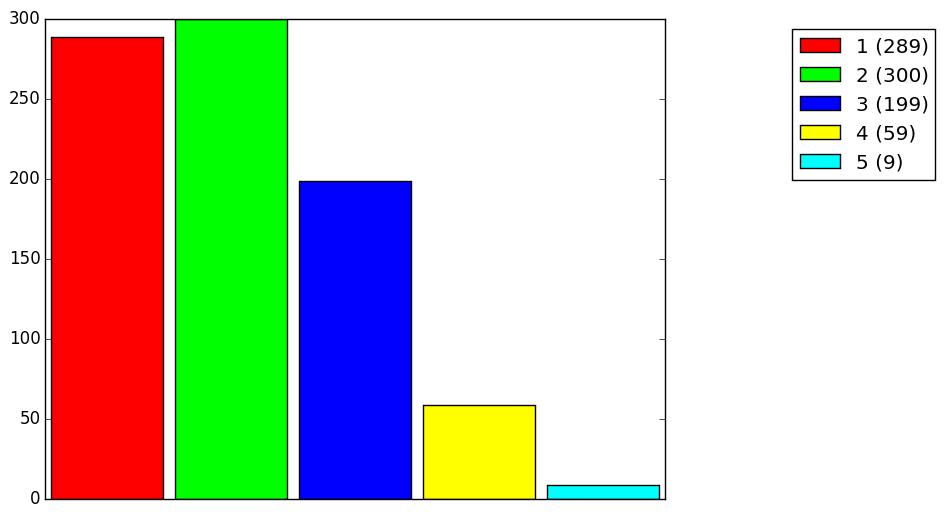
\includegraphics[scale=0.55]{images/datensicher}\\
\caption{Meine Daten sind bei Google sicher}\label{datensicher}
\end{figure}
\begin{figure}[H]
\centering
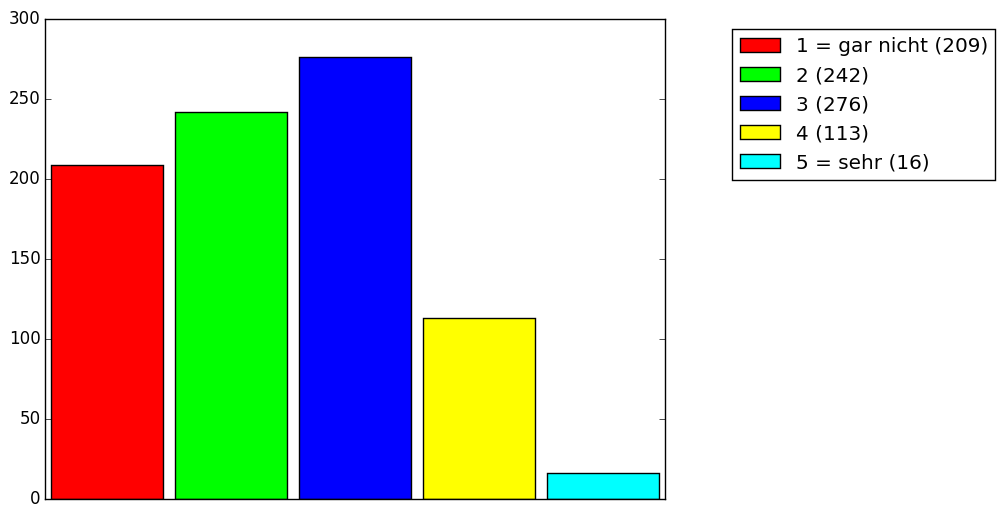
\includegraphics[scale=0.55]{images/vertrauen}\\
\caption{Wie stark vertrauen Sie Google}\label{vertrauen}
\end{figure}
\begin{table}
	\begin{tabular}[]{ c || c | c | c | c | c | c}
	& \multicolumn{5}{c}{Ich vertraue darauf, dass diese Firma meine Privatsphäre schützt:}\\
	& Microsoft & Facebook & Apple & Google & Paypal & Amazon\\ \hline \hline
	1 &191 (22,3\%)&587 (68,6\%)&323 (37,7\%)&295 (34,5\%)&131 (15,3\%)&186 (21,7\%)\\ \hline
	2 &197 (23,0\%)&176 (20,7\%)&220 (25,7\%)&269 (31,4\%)&123 (14,4\%)&197 (23,0\%)\\ \hline
	3 &250 (29,2\%)&56 (6.5\%)&185 (21,6\%)&170 (19,9\%)&168 (19,6\%)&217 (25,4\%)\\ \hline
	4 &166 (19,4\%)&21 (2,5\%)&90 (10,5\%)&88 (10,3\%)&220 (25,7\%)&171 (20,0\%)\\ \hline
	5 &52 (6,1\%)&16 (1,9\%)&38 (4,4\%)&34 (4,0\%)&214 (25,0\%)&85 (9,9\%)\\ \hline
	\end{tabular}
	\caption{Ich vertraue darauf, dass diese Firma meine Privatsphäre schützt}\label{vertrauenothers}
\end{table}

Zum Wahrgenommenen Risiko für die Privatsphäre \ref{itm:Kat3} gibt es meist sehr eindeutige Antworten. \glqq Sehen Sie das Nutzen von personenbezogenen Daten seitens Google als Vorteil für Sie?\grqq\ beantworteten nur 11,5\% der Teilnehmer mit Ja. Mit 65,8\% sind weit mehr als die Hälfte der Nutzer der Meinung, dass es keine Vorteile bietet.
Diejenigen die mit Ja geantwortet haben nennen zum Großteil die angepassten Suchergebnisse als Vorteil. Auch die angepasste Werbung wird häufig genannt.

85,9\% der Teilnehmer ist der Meinung, dass sie sich bei der Nutzung von Google Diensten gegenüber Google nicht anonym fühlen. Nur 6,4\% fühlen sich anonym.
Grafik \ref{possibilities} zeigt auf, ob die Teilnehmer glauben, dass Google ihnen ausreichend Möglichkeiten gibt um ihre Privatsphäre zu schützen. 1 entspricht wieder gar nicht, 5 sehr. Es zeigt, dass sich der Großteil der Teilnehmer auf der unteren Hälfte befindet. Antworten 3,2 und 1 belaufen sich zusammen auf 91,1\%. 

\begin{figure}[H]
\centering
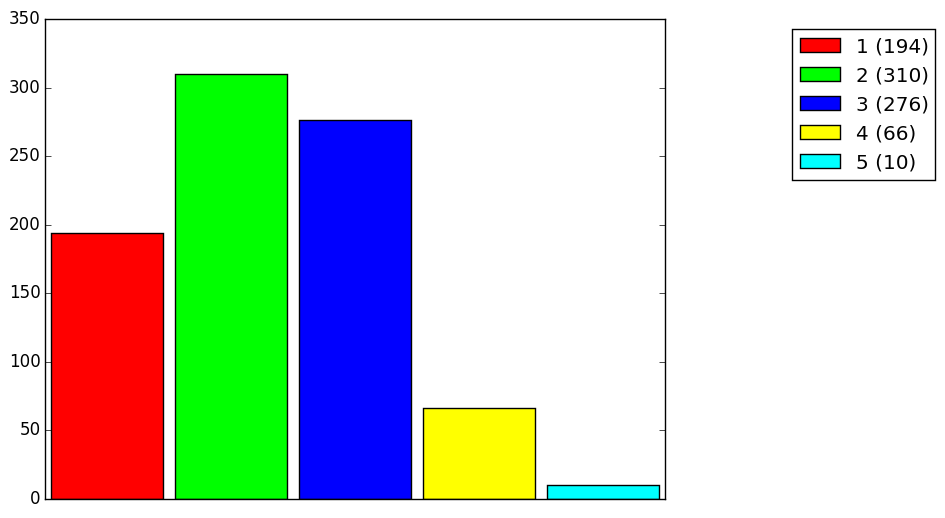
\includegraphics[scale=0.55]{images/possibilities}\\
\caption{Google bietet mir ausreichend Möglichkeiten meine Privatsphäre zu schützen.}\label{possibilities}
\end{figure}

Die Fragen zu den Schutzmaßnahmen \ref{itm:Kat5} wurden teilweise nur von sehr wenigen Teilnehmern beantwortet, da die Fragen abhängig von den Antworten anderer Fragen waren. Deswegen gibt es bei \glqq Haben Sie diese Einstellung aktiv?\grqq\ im Bezug auf \glqq Gibt es eine Einstellung die es Google verbietet Ihren Google+ Namen zusammen mit Ihrem Foto zu Werbezwecken zu verwenden?\grqq\ insgesamt nur sieben Antworten. Von diesen sieben Antworten sind allerdings fünf \glqq Ja\grqq\ , nur eine \glqq Nein\grqq\ .

Bei \glqq Haben Sie Maßnahmen unternommen um anonym gegenüber Google zu sein? Wenn ja, welche?\grqq\ gab es insgesamt 55 Antworten, von denen 21 mit Ja und 28 mit Nein geantwortet haben. 

Mehr Antworten gibt es wieder bei \glqq Würden Sie Ihren Google Account löschen um an Privatsphäre zu gewinnen?\grqq\ . Hierbei haben von allen Teilnehmern 52,1\% mit Nein geantwortet. Die restlichen knapp 50\% der Teilnehmer teilen sich mit 27,7\% zu Ja und 20,2\% zu Nein auf.

Tabelle \ref{changedprivacy} zeigt auf, bei welchem Google Dienst die Teilnehmer der Umfrage bereits Einstellungen für die Privatsphäre geändert haben. Die Option \glqq Sonstiges\grqq\ wurde zum Großteil dazu genutzt mit \glqq keinem\grqq\ zu antworten.
\begin{table}
	\begin{tabular}[]{ c || c | c }
	\multicolumn{3}{c}{Bei welchem Google Dienst haben Sie bereits Privatsphäre Einstellungen geändert?}\\\hline
	Dienst & Anzahl (absolut) & Anzahl (relativ)\\\hline\hline
	Google Suche & 251 & 29,3\%\\
	Google Mail & 262 & 30,6\%\\
	Android & 369 & 43,1\%\\
	Google Chrome & 204 & 23,8\%\\
	Youtube & 331 & 38,7\%\\
	Google Maps & 101 & 11,8\%\\
	Google+ & 131 & 15,3\%\\
	Picasa & 32 & 3,7\%\\
	Hangouts & 26 & 3,0\%\\
	Google Docs & 40 & 4,7\%\\
	Google Kalender & 75 & 8,8\%\\
	Sonstiges & 44 & 5,1\%\\
	\end{tabular}
	\caption{Bei welchem Google Dienst haben Sie bereits Privatsphäre Einstellungen geändert?}\label{changedprivacy}
\end{table}

Das letzte Konstrukt, \glqq Bewusstsein über das Aufgeben der Privatsphäre\grqq\ \ref{itm:Kat4}, zeigt sehr interessante Ergebnisse. Zum Beispiel wollen 596 der 735 Teilnehmer, denen die Frage gezeigt wurde, gegenüber Google gerne anonym sein.

Grafik \ref{giveinfo} zeigt auf, dass die Mehrzahl der Teilnehmer glaubt, wenige Daten über das private Leben im Internet herauszugeben. Dies steht im Konflikt mit der Frage nach \glqq Ich denke, Google weiß folgendes über mich:\grqq\ , bei der 89,7\% der Teilnehmer angaben, Google wüsste ihren Namen, 83,6\% sind der Meinung Google wüsste sogar ihren Wohnort. Interessen und derzeitiger Aufenthaltsort sind mit 76,1\% und 65,8\% auch sehr häufig angewählt worden. Im \glqq Sonstiges\grqq\ Bereich wurde oft \glqq IP Adresse\grqq\ und \glqq Sexuelle Interessen\grqq\ genannt.

Die Frage \glqq Durch die Nutzung von Google Diensten gebe ich zu viel meiner Privatsphäre auf\grqq\ wurde von 34,9\% der Teilnehmern mit der mittleren der fünf Auswahlmöglichkeiten beantwortet. Vier und Fünf, die Antworten die mit \glqq zu viel\grqq\ betitelt waren, wurden zusammen von 36,1\% der Teilnehmern gewählt, wohingegen die andere Seite von 29,0\% gewählt wurden. Hier ist also eine leichte Tendenz zur Seite \glqq zu viel\grqq\ zu sehen.

\begin{figure}[H]
\centering
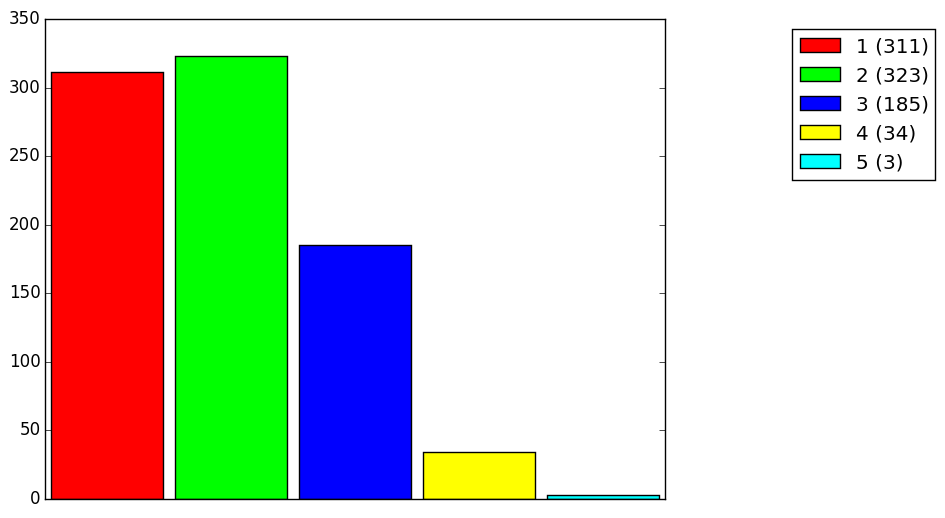
\includegraphics[scale=0.55]{images/giveinfo}\\
\caption{Wie viele Informationen über Ihr privates Leben gegen Sie im Internet heraus?}\label{giveinfo}
\end{figure}

\section{Verwendete Tests}
Zur Bestimmung von Korrelationen und der statistischen Signifikanz wurden die folgenden Methoden und Formeln verwendet:

\subsection{Chi-Quadrat}
\label{chisquared}
Der $\chi$-Quadrat-Test ist eine Methode um eine Beziehung zwischen zwei Variablen aufzustellen, die mindestens ein Nominalskalenniveau aufweisen.
Hierfür wird häufig die Darstellung einer Kreuztabelle verwendet, wie sie auch schon in dieser Arbeit des öfteren verwendet wurde.

Um nun eine Korrelation und ihre Signifikanz zu bestimmen kann der $\chi$-Quadrat-Test verwendet werden. Die Formel dafür lautet:\\
$\chi^2 = \sum_{j=1}^m \frac{(f_{b(j)} - f_{e(j)})^2}{f_{e(j)}}$ (\citet{statistikeinfuehrung})\\
wobei $m$ der Anzahl der Zellen entspricht, $f_b$ die beobachteten Häufigkeiten und $f_e$ die erwarteten Häufigkeiten sind.

Um nun eine Signifikanz zu bestimmen muss noch ein Koeffizient berechnet werden. In den meisten Fällen kann hier der Phi-Koeffizient verwendet werden. Er berechnet sich nach:\\
$\phi = \frac{a \cdot d - b \cdot c}{\sqrt{(a+c) \cdot (b+d) \cdot (a+b) \cdot (c+d)}}$\\
wobei $a, b, c, d$ den jeweiligen Zellenhäufigkeiten entsprechen.

Die kürzere Variante um den Phi-Koeffizienten zu berechnen ist: $\phi = \sqrt{\frac{\chi^2}{n}}$

Als weitere Methode tritt der Zusammenhangskoeffizient V nach Cramer auf. Er wird durch die folgende Formel bestimmt: $V = \sqrt{\frac{\chi^2}{n \cdot (min(l,k) - 1)}}$. Die Variable k entspricht hier der Anzahl der Kategorien der Zeilenvariablen, l der Anzahl der Kategorien der Spaltenvariablen. Diese Berechnung hat den Vorteil, dass sie auch bei Tabellen die größer als 2x2 sind funktioniert.

Sämtliche Korrelationen werden nach \citet{statistikeinfuehrung} anhand Tabelle \ref{correlationrelevance} bewertet.

\begin{table}
	\begin{tabular}[]{ c | c }
	$|r|$ & Stärke des Zusammenhanges\\\hline\hline
	$0,00 \leq r < 0,10$ & Kein Zusammenhang\\\hline
	$0,10 \leq r < 0,30$ & Geringer Zusammenhang\\\hline
	$0,30 \leq r < 0,50$ & Mittlerer Zusammenhang\\\hline
	$0,50 \leq r < 0,70$ & Hoher Zusammenhang\\\hline
	$0,70 \leq r < 1,00$ & Sehr hoher Zusammenhang\\\hline
	\end{tabular}
	\caption{Stärke des Zusammenhanges}\label{correlationrelevance}
\end{table}

\section{Hypothesen}
\textit{Je aktiver eine Person Google nutzt, desto mehr Kenntnisse über Googles Datenschutz bekommt sie. (H1, \ref{itm:H0})}

Hier lassen sich einige Korrelationen aufstellen. So zeigt zum Beispiel Tabelle \ref{4ssearchads}, dass 14,1\% derjenigen, die die Google Suche am aktivsten Nutzen, auf die Frage, ob Google zugeschnittene Werbung anbietet, mit \glqq Nein\grqq\ oder \glqq Weiß nicht\grqq\ geantwortet haben. Dieser prozentuale Wert entspricht exakt dem äquivalenten Wert in der Spalte \glqq Gesamt\grqq\ .

Tabelle \ref{4ssearchsearch} zeigt ein ähnliches Bild, es ist allerdings eindeutig ersichtlich, dass in der Frage nach den zugeschnittenen Suchergebnissen 40 Teilnehmer weniger mit \grqq Ja\glqq\ geantwortet haben. Diese 40 fehlen offensichtlich im Bereich derjenigen, die die Google Suche sehr aktiv nutzen, was allerdings nur 4\% der Teilnehmer sind und somit die Hypothese nicht widerlegt.

Die prozentualen Anteile von derjenigen, die mit Ja geantwortet haben zur Gesamtzahl jeder Zeile von Tabelle \ref{4ssearchsearch} belaufen sich auf: 1: 82,4\%, 2: 93,8\%, 3: 71,4\%, 4: 80,4\%, 5: 80,7\% und im Gesamten 81,0\%. Hierdurch lässt sich also keine Beziehung zwischen der Nutzung und den Kenntnissen über Google Dienste und Privatsphäre aufzeigen.

\begin{table}
	\begin{tabular}[]{ l c | c | c | c | c }
	& & \multicolumn{3}{c |}{Bietet Google auf Nutzer zugeschnittene} &\\
	& & \multicolumn{3}{c |}{Werbung an?} &\\ \hline
	& & Ja & Nein & Weiß nicht & Gesamt\\ \hline
	[Google Suche] Wie aktiv& 1 & 30 & 0 & 4 & 34\\
	nutzen Sie die folgenden& 2 & 32 & 0 & 0 & 32\\
	Google Dienste?& 3 & 18 & 1 & 2 & 21\\
	(1: gar nicht, 5: sehr)& 4 & 113 & 5 & 20 & 138\\
	& 5& 542 & 20 & 69 & 631\\ \hline
	Gesamt & & 735 & 26 & 95 & 856\\ \hline
	\end{tabular}
	\caption{Wie aktiv nutzen Sie die folgenden Google Dienste? [Google Suche] x Bietet Google auf Nutzer zugeschnittene Werbung an?}\label{4ssearchads}
\end{table}
\begin{table}
	\begin{tabular}[]{ l c | c | c | c | c }
	& & \multicolumn{3}{c |}{Bietet Google auf Nutzer zugeschnittene} &\\
	& & \multicolumn{3}{c |}{Suchergebnisse an?} &\\ \hline
	& & Ja & Nein & Weiß nicht & Gesamt\\ \hline
	[Google Suche] Wie aktiv& 1 & 28 & 2 & 4 & 34\\
	nutzen Sie die folgenden& 2 & 30 & 0 & 2 & 32\\
	Google Dienste?& 3 & 15 & 2 & 4 & 21\\
	(1: gar nicht, 5: sehr)& 4 & 111 & 5 & 22 & 138\\
	& 5 & 509 & 31 & 91 & 631\\ \hline
	Gesamt & & 693 & 40 & 123 & 856\\ \hline
	\end{tabular}
	\caption{Wie aktiv nutzen Sie die folgenden Google Dienste? [Google Suche] x Bietet Google auf Nutzer zugeschnittene Suchergebnisse an?}\label{4ssearchsearch}
\end{table}
Tabelle \ref{4samountdelete} zeigt allerdings eine Beziehung auf. Die Teilnehmer die einen oder gar keinen Google Account haben sind sich sehr unsicher darüber ob es die Möglichkeit gibt den Account zu löschen, 85,3\% der Teilnehmer mit keinem Google Account haben hier mit \glqq Weiß nicht\grqq\ geantwortet. Das ist verständlich, wenn man keinen Account hat ist es auch nicht wichtig zu wissen ob man ihn wieder entfernen könnte.

Aber vor allem bei den Teilnehmern mit einem Google Account zeigen sich große Defizite auf - 63,5\% von ihnen wissen nicht, ob man den Account löschen kann. Je mehr Accounts ein Teilnehmer besitzt desto sicherer ist er sich, dass er den Account auch wieder löschen kann. Dieser Wert steigt von 31,4\% für Teilnehmer mit einem Account, über 47,7\% bei einem Account auf 56,9\% für Teilnehmer mit mehr als 2 Accounts. Hier ist eine Korrelation zu erkennen welche die Hypothese unterstützt, dass mehr Nutzung mehr Wissen entspricht.

Diese Korrelation wurde mit dem $\chi$-Quadrat-Test (\ref{chisquared}) geprüft. Hierbei ergibt sich, dass nach Tabelle \ref{correlationrelevance} nur ein geringer statistischer Zusammenhang besteht.

Die aufgeführten Argumente lassen darauf schließen, dass die Hypothese zwar nicht statistisch signifikant angenommen werden kann, aber es dennoch Indizien gibt, dass Teilnehmer, die Google aktiver nutzen in einigen Bereichen mehr über den Datenschutz im Bezug auf Google wissen.

\begin{table}
	\begin{tabular}[]{ l c | c | c | c | c }
	& & \multicolumn{3}{c |}{Bietet Google die Möglichkeit den eigenen} &\\
	& & \multicolumn{3}{c |}{Account zu löschen?} &\\ \hline
	& & Ja & Nein & Weiß nicht & Gesamt\\ \hline
	Wie viele Google& 0 & 13 & 4 & 99 & 116\\
	Accounts haben Sie?& 1 & 174 & 28 & 352 & 554\\
	& 2 & 61 & 9 & 58 & 128\\
	& mehr als 2 & 33 & 6 & 19 & 58\\
	Gesamt & & 281 & 47 & 528 & 856\\ \hline \hline
	Chi-Quadrat: 64,1 & & & & &\\
	Likelihood-Quotient: 67,5&&&&&\\
	Nominal bzgl. Phi: 0,27&&&&&\\ \hline
	\end{tabular}
	\caption{Wie viele Google Accounts besitzen Sie? x Bietet Google die Möglichkeit den eigenen Account zu löschen?}\label{4samountdelete}
\end{table}


TODO AREA:\\
"Meine Daten sind bei Google sicher" und "Durch die Nutzung von Google Diensten gebe ich zu viel von meiner Privatsphäre auf" korrelieren nur relativ schwach mit r(854) = -0.29. Es ergibt sich also eine indirekte Korrelation, die allerdings nur sehr schwach ist. Eine leichte Tendenz ist dennoch vorhanden.

\section{Forschungsfragen}

\section{Sonstiges}
